% \documentclass{beamer}
% \usetheme{default} 
% 
% \setbeamercolor{structure}{fg=green!40!black} 
% \usebackgroundtemplate{
%     \centering
\includegraphics[width=\paperwidth,height=\paperheight]{images/android_wall}
% }
% \setbeamertemplate{navigation symbols}{}
% 
% \usepackage[polish]{babel}
% \usepackage[utf8x]{inputenc}
% \usepackage{t1enc}
% \usepackage{default}
% \usepackage{listings}
% 
% \lstset{language=java, basicstyle=\small, commentstyle=\color{gray}}
% \lstset{frame=single}
% 
% \usefoottemplate{
%   \vbox{
%     \tinycolouredline{structure!25}{
%       \color{black}\textbf{	
%         \insertshortauthor\hfill
%         Android @ Szczecin 2011
%       } 
%     }
% %    \tinycolouredline{structure}{
% %      \color{white}\textbf{\insertshorttitle}\hfill
% %    } 
%   }
% }
% 
% \title{Android @ Szczecin \\ 2011}
% \author{Konrad Malawski \\ konrad.malawski@java.pl}
% 
% \begin{document}







\begin{frame}
\titlepage
\end{frame}

\begin{frame}
 \begin{center}
  \Huge{Hello!}
 \end{center}

\end{frame}


% \begin{frame}
%  \frametitle{me.about();}
%  \centering
%  Konrad Malawski \\
%  Lunar Logic Polska \\
%  _\\
%  PolishJUG \\ 
%  GeeCON\\
%  KrakówGTUG\\
%  _\\
%  twitter: @ktosopl\\
%  github: ktoso\\
%  blog: blog.project13.pl\\
% \end{frame}

\begin{frame}
  \centering
  
\includegraphics[width=\textwidth,height=\textheight]{images/about_me_slide}
\end{frame}

\begin{frame}
 \begin{center}
  \Huge{You?}
 \end{center}

\end{frame}



\begin{frame}\frametitle{Architektura}

  \begin{figure}[t]
    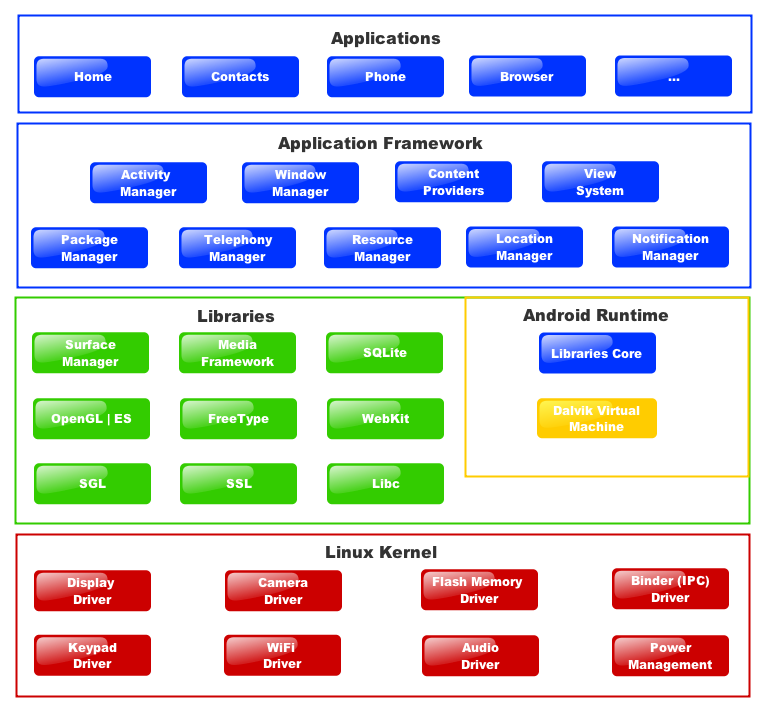
\includegraphics[height=0.62\textheight,keepaspectratio=true,clip=true]{images/platform}
    \caption{Architektura systemu Android}
  \end{figure}

\end{frame}

\begin{frame}\frametitle{Słowa na dziś:}
 \begin{itemize}
  \item \Huge{Application}
  \item \Huge{Activity}
  \item \Huge{View}
  \item \Huge{Service}
  \item \Huge{Intent}
  \item \_\_\_\_\_\_\_\Huge{Manager}
 \end{itemize}
\end{frame}

\begin{frame}
\begin{center}
 \Huge{The ,,Glue'':}\\ 
 \Huge{AndroidManifest.xml}
\end{center}

\end{frame}


\begin{frame}[fragile]\frametitle{AndroidManifest.xml}
\begin{lstlisting}
<manifest xmlns:android="http://..."
     package="pl.project13.android.github.notify"
     android:versionCode="1"
     android:versionName="1.0">

  <application android:name=".guice.GitHubNotifyApplication"
               android:label="@string/app_name"
               android:icon="@drawable/icon"
               android:debuggable="true"
               android:hardwareAccelerated="true">

    <activity android:name=".activity.WatchPreferencesActivity"
              android:icon="@drawable/icon"
              android:label="GitHub Notify">
      <intent-filter>
        <action android:name="android.intent.action.MAIN"/>
        <category android:name="android.intent.category.LAUNCHER"/>
      </intent-filter>
    </activity>
\end{lstlisting}
\end{frame}

\begin{frame}[fragile]\frametitle{AndroidManifest.xml}
\begin{lstlisting}
    <service android:name=".service.NewCommitNotifierService"/>
  </application>

  <!-- PERMISSIONS -->
  <uses-sdk android:minSdkVersion="6"
            android:targetSdkVersion="11"/>

  <uses-permission android:name="android.permission.INTERNET"/>
  <uses-permission android:name="android.permission.ACCESS_NETWORK_STATE"/>
  <uses-permission android:name="android.permission.RECEIVE_BOOT_COMPLETED"/>
</manifest>
\end{lstlisting}
\end{frame}

% przegląd ACTIVITIES
\begin{frame}\frametitle{Activity lifecycle}
 \begin{figure}[ct]
  \centering
  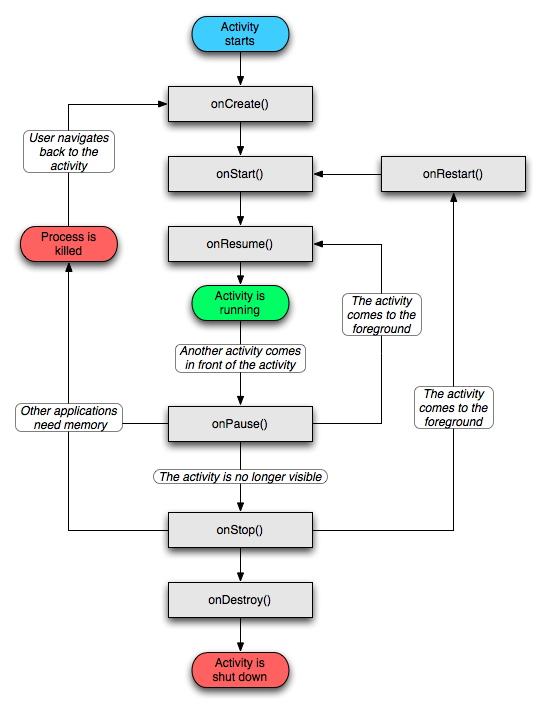
\includegraphics[height=\textheight]{images/activity_lifecycle}
 \end{figure}
\end{frame}

\begin{frame}[fragile]\frametitle{Activity}
Wołany gdy Activity jest tworzona po raz pierwszy.
\begin{lstlisting}
  public class MainActivity extends Activity {
    public void onCreate(Bundle savedState) {
      /**/
    }
  }
\end{lstlisting}

\end{frame}

% TODO TROSZKE WIwcej o activities

% przegląd VIEWS
\begin{frame}[fragile]\frametitle{LinearLayout + EditText z wrap\_content}
 \begin{columns}
  \column{.7\textwidth}
  \begin{verbatim}
<LinearLayout
 android:id="@+id/root_layout"
 android:layout_width="fill_parent"
 android:layout_height="fill_parent"
 android:orientation="vertical">
  <!-- ... -->

  <TextView android:id="..." ... />
  <EditText android:id="..."
   android:layout_width="fill_parent"
   android:layout_height="wrap_content" 
  />
</LinearLayout>

  \end{verbatim}
  \column{.4\textwidth}
  \begin{figure}
   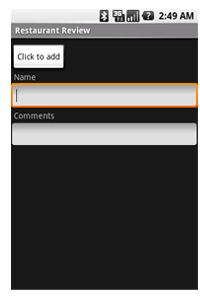
\includegraphics[width=.7\textwidth]{images/linearlayout_wrap}   
  \end{figure}

 \end{columns}
\end{frame}

\begin{frame}[fragile]\frametitle{LinearLayout + EditText z fill\_parent}
 \begin{columns}
  \column{.7\textwidth}
  \begin{verbatim}
<LinearLayout
 android:id="@+id/root_layout"
 android:layout_width="fill_parent"
 android:layout_height="fill_parent"
 android:orientation="vertical">
  <!-- ... -->

  <TextView android:id="..." ... />
  <EditText android:id="..."
   android:layout_width="fill_parent"
   android:layout_height="fill_parent" 
  />
</LinearLayout>

  \end{verbatim}
  \column{.4\textwidth}
  \begin{figure}
   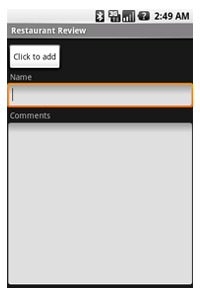
\includegraphics[width=.7\textwidth]{images/linearlayout_fill}   
  \end{figure}

 \end{columns}
\end{frame}

\begin{frame}[fragile]\frametitle{Panowanie nad Layoutami}
\begin{itemize}
 \item Istnieje jeszcze \textbf{match\_parent}, pojawił się w nowszych wersjach Android, jest analogiczny do fill\_parent.
 \item W przypadku gdy chcemy ustalać ''jaką część widoku ma zajmować pewien element'', korzystamy z \textbf{android:layout\_weight}, przyjmuje on liczby \textit{(default = 1)}.
\end{itemize}
\end{frame}

\begin{frame}\frametitle{Ważne ViewGroups:}
\begin{itemize}
 \item \textbf{FrameLayout} - Layout dla tylko jednego elementu, najprostszy
 \item \textbf{LinearLayout} - Wystarczający dla prostych widoków, kombinowanie kilku LinearLayout daje przyjemne efekty
 \item \textbf{ListView} - Sam dba o scrollowanie
 \item \textbf{TabHost} - Może mieć zakładki
 \pause \item \textbf{Spinner}, \textbf{Gallery}, \textbf{GridView}, \textbf{RelativeLayout}, \textbf{ScrollView}, \textbf{SurfaceView}, \textbf{TableLayout}, \textbf{ViewFlipper}, \textbf{ViewSwitcher}...
\end{itemize}
\end{frame}


% Resources
\begin{frame}\frametitle{R, as in Resource}  
\begin{center}
 \Huge{\textbf{R}}
\end{center}
\end{frame}

\begin{frame}[fragile]\frametitle{R, as in Resource}
 \begin{lstlisting}
package pl.project13;

public final class R {
    public static final class drawable {
        public static final int icon=0x7f020000;
    }
    public static final class id {
        public static final int login=0x7f050000;
    }
    public static final class layout {
        public static final int main=0x7f030000;
    }
    public static final class string {
        public static final int app_name=0x7f040000;
    }
}
 \end{lstlisting}
\end{frame}

\begin{frame}[fragile] \frametitle{R, as in Resource}  
 Dodanie elementu id \textbf{wewnątrz widoku}, poprzez \textbf{+@id/}
\begin{lstlisting}
 <EditText android:id="@+id/login" ... />
\end{lstlisting}

\pause

Spowoduje wygenerowanie pola w klasie \textbf{R}:
\begin{lstlisting}
public final class R {
  public static final class id {
    public static final int login = 0x7f050000;
  }
}
\end{lstlisting}

\pause

A skorzystamy z niego w np. \textbf{Activity}:
\begin{lstlisting}
 EditText mLogin = findById(pl.project13.R.id.login);
\end{lstlisting}
\end{frame}

\begin{frame}[fragile]\frametitle{Strings as Resources}
\begin{figure}
\title{res/layouts/main.xml}
\begin{lstlisting}
<TextView android:layout_height="fill_parent"
          android:layout_width="fill_parent"
          android:text="Witaj swiecie!"
       />
\end{lstlisting}
\end{figure}

Mieszanie treści z layoutem jest złym pomysłem.
\end{frame}

\begin{frame}[fragile]\frametitle{Strings as Resources}
\begin{figure}
\title{res/layouts/main.xml}
\begin{lstlisting}
<TextView android:layout_height="fill_parent"
          android:layout_width="fill_parent"
          android:text="@string/hello_world"
       />
\end{lstlisting}
\end{figure}

\begin{figure}
 \title{res/values/strings.xml}
\begin{lstlisting}
<resources>
  <string name="hello_world">Witaj swiecie!</string>
</resources>
\end{lstlisting}
\end{figure}

(Tip: W intellij piszemy \textit{@string/hello\_world} a następnie ALT+ENTER, aby utworzyć zasób w odpowiednim miejscu.)
\end{frame}

\begin{frame}[fragile]\frametitle{Proste I18N (i nie tylko) dzięki klasyfikatorom}

\centering
\ttfamily 
res/values-\textbf{pl}/strings.xml

\begin{figure}
\begin{lstlisting}
<resources>
  <string name="hello_world">Witaj swiecie!</string>
</resources>
\end{lstlisting}
\end{figure}

\centering
\ttfamily 
res/values-\textbf{en}/strings.xml
\begin{figure}
\begin{lstlisting}
<resources>
  <string name="hello_world">Hello world!</string>
</resources>
\end{lstlisting}
\end{figure}


\end{frame}


\begin{frame}\frametitle{R, tips and tricks}
\begin{itemize}
 \item nazwy wykorzystywane dla np. ID \textbf{nie muszą} być unikalne, @+id/login raz może oznaczać ten EditText a raz TextView.
       Rozwiązywane jest do wedle 'na czym wołany jest findById'.
 \pause \item Korzystamy raczej z 'notacji\_z\_podkresleniami\_tutaj'
 \pause \item W kontekście gdzie nie masz \textbf{findById}, skorzystaj z \textbf{android.content.res.Resources.getSystem().get\_\_\_\_\_()}
\end{itemize}
\end{frame}

\begin{frame}\frametitle{Zadanie: Hello Szczecin!}
\begin{itemize}
 \item Prosty widok z przyciskiem oraz tekstem oraz polem tekstowym na czyjeś imię
 \item Ma być możliwe podanie swojego imienia, wtedy text po wciśnięciu przycisku ma wyglądać ,,Hello \_\_\_\_!''
 \item tip: korzystamy z \textbf{res/values/strings.xml} oraz \textbf{res/layouts/main.xml}
 \item tip: Przydadzą się widżety: TextView, Button, EditText
 \pause \item \textbf{Uwaga! Skorzystamy z \textbf{Robolectric} to \textit{TDD}* aplikacji Androiowej!}
\end{itemize}

* TDD - Test Driven Development\\
Tak tak, ponieważ zwyczajny hello world byłby nudny! :-)\\
\textit{Testy są już dla Was przygotowane.}
\end{frame}

\begin{frame}[fragile]\frametitle{Testowanie a sprawa Androida}
Jest pewien problem z 'zwyczajnym testowaniem' aplikacji androidowych... Wcześniej czy później wpadnie się na:
 
 \begin{figure}[ch]
  \verb|java.lang.RuntimeException: Stub!|
 \end{figure}

\begin{figure}[hc]

\includegraphics[width=0.25\textwidth]{images/robolectric}\\
\centering
http://pivotal.github.com/robolectric/index.html
\end{figure}

Robolectric zastępuje implementacje rzucające te wyjątki domyślnymi (\verb|return 0 / null|).
\end{frame}

\begin{frame}[fragile]\frametitle{Plain Old Testing}
Jakby ktoś faktycznie chciał rzeźbić bardziej niskopoziomowo swoje testy,
oto jak to zrobić: 

\begin{verbatim} 
http://developer.android.com/resources/
                             tutorials/testing/
                             activity_test.html
\end{verbatim}
\end{frame}

\begin{frame}[fragile]\frametitle{Zadanie: Hello Szczecin!}
\begin{itemize}
 \item Prosty widok z przyciskiem oraz tekstem oraz polem tekstowym na czyjeś imię
 \item Ma być możliwe podanie swojego imienia, wtedy text po wciśnięciu przycisku ma wyglądać ,,Hello \_\_\_\_!''
 \item tip: korzystamy z \textbf{res/values/strings.xml} oraz \textbf{res/layouts/main.xml}
 \item tip: Przydadzą się widżety: TextView, Button, EditText
 \textbf{Skorzystamy z \textbf{Robolectric} to \textit{TDD}* aplikacji Androiowej!}
\end{itemize}

\begin{verbatim}
 git clone git@github.com:ktoso/szczecin-android.git
 cd szczecin-android/projects/simple-button
\end{verbatim}

\end{frame}





% 
% 
% \end{document}